\documentclass{article}
\usepackage[margin=1in]{geometry}
\usepackage{graphicx}
\usepackage{float}
\usepackage{listings}
\title{ECS 145 Term Project Winter 2020}
\author{Atul Jayaram, Han Nguyen, Jamie Arrillaga, Zachary Anway}
\date{\today}
\begin{document}
\maketitle

\newpage
\tableofcontents
\newpage

\section{Group Dynamics}
\subsection{Meeting 1: Designing Detailed Specs}
Our first group meeting was centered on adding rigor to the specs, particularly how we would like to handle implementing certain features. The details of how each of these are implemented are discussed in section 2. This was also the point where we discussed how to
\subsubsection{Design Choice 1: Using terminal vs GUI}
We briefly considered the possibility of having a GUI that allows the user to have buttons for zooming, seeing animations, etc. However, besides requiring more time, we figured a simple CLI based approach would allow the user to quickly run options through the keyboard. This decision is further re-enforced by the fact that the feature set is small enough that a GUI is not needed to introduce intuitiveness to the interface; the interface is easy enough to figure out.
\subsubsection{Design Choice 2: \textit{Everything} is handled through the terminal}
There are two ways to handle closing a graph window that we have found in R: wait for a newline character to be entered by the user and call graphics.off() or wait for the user to close it themselves. We went with the first option, because it is consistent with design choice 1. We want all interfacing done through the keyboard, not having the user scrolling with the mouse in order to close a graph. This allows for more streamlined interfacing with our library.
\subsubsection{Design Choice 3: Using external libraries}
We opted to use external libraries to implement animation, since all online research pointed toward using external libraries. That said, for all other features, we decided to avoid using other packages in order to restrict the amount of dependencies our project required. This was also a effort to reduce the amount of potential errors that could occur when integrating many libraries at once.

\subsection{Meeting 2: Group Programming and Feature Delegations}
\subsubsection{Baseline Implementations}
Now that we were aware of how we wanted to go about the project, we needed to start coding. Zach had written a simple skeleton that grabs input and execute a feature based on their entry. We gathered around a single machine and implemented the features one by one, with each member contributing ideas about how to implement a given feature. By the end, each feature had a rudimentary implementation. We then looked at each feature and critiqued what could be better. We observed the following: \\
1. Zoom out always zoomed back out to the entire data set. Atul suggested a stack based approach that the last zoom in is remembered, so that when a zoom out occurs, the user is given the option to zoom all the way out or to zoom out to the previously selected subset of the data set. This was originally done with the idea that we would have a default zoom amount if the user never entered any parameters. However, Atul realized that a stack based approach wasn't necessary. We could simply keep a copy of the original data set and all operations would be made on that copy. Additionally, we would always allow the user to set the zooming in/out scope parameters. This results in better control for the user, as well as less complex code. In the end, Atul just theorized that certain checks would need to be made to ensure valid zoom operations, but otherwise the main idea was solid.\\
2. We all observed that the animations would demand more research into the gganimate library, as the result we had would consistently generate a blank screen.\\
3. Input validation was lacking. We recognized that all features we implemented would need some sort of validation in order to prevent crashes on bad input.

\subsubsection{Delegations}
While we had effectively finished the project in one sitting, it was rough and demanded that each feature be polished/expanded and then underwent an aggressive refactor. We all discussed and then delegated the following roles:\\
1. Zach would implement the S3 object with plot, summary, and print. This includes letting the user specify which tunings they want to use.\\
2. Jamie would dig into the gganimate documentation and figure out how to implement animations.\\
3. Atul would implement the zooming feature.\\
4. Han was responsible for implementing the graph overlay feature for when twoAtATime is specified in the function call.\\
5. Upon completion and merge of everyone's code, everyone was responsible for testing all features.

\subsection{Following Meetings}
All following meetings and discussion were done though Slack. We set up threads to discuss errors we were encountering, for questions relating to someone's code, and for general discussion of our progress. Everyone was responsive, so this dynamic was able to allow us to work remotely until the completion of the project.

\section{Feature Set}
\subsection{Option 1: Setting Tuning}
The user can select a new tuning parameter, being prompted to enter one until a positive integer is provided. This will then be used in all future graph displays until the tuning is changes again.
\subsubsection{Overlaying Graphs}
If the function is called with twoAtATime parameter set to TRUE, then the previous tuning is saved and a graph with the selected tuning is displayed over the graph with the previous tuning.

\subsection{Option 2: Zoom In}
The user is allowed to select a subset of the data to display. The only restrictions provided on the user are that the indices selected are in range.

\subsection{Option 3: Zoom Out}
Zoom out provided two options: \\
1. The user can zoom all the way out (look at the entire dataset).\\
2. Zoom out to a valid subset.  \\

The only restrictions provided on the user once again are that the indices selected are in range.

\subsection{Option 4: Running Animations}
The user is allowed to select a start and end tuning. An animation is then ran that shows how the graph changes as the tuning is incremented, until the end tuning is reached.

\subsection{Option 5: Building Graphs}
The user is prompted to enter a tunings (verified to be integers), until the user enters 'q'. Then an S3 object is constructed and it returned, ending the function call.

\subsection{Option 6: Re-displaying graph}
Reopens the current graph.

\section{densEst Composition, Functions}
\subsection{densEst fields}
The densEst object has the following fields:\\
1. estMethod: either 'hist' or 'density'. Specifies what type of graph should be used.\\
2. dataVector: vector containing the data to be graphed. \\
3. tunings: integer vector containing all the tunings to be iteratively applied to dataVector when densEst object is plotted. 
\subsection{print}
Print will print out the list of tunings, as well as the estMethod. If the user provides optional parameter printVector = TRUE, then the dataVector is also printed.

\subsection{summary}
Summary outputs some basic statistics and info about the dataset and tunings. The following will be printed:\\
1. estMethod\\
2. mean of dataVector\\
3. standard deviation of dataVector\\
4. mean of tunings\\
5. standard deviation of tunings

\subsection{plot}
Plot will graph the data vector according to estMethod. The tunings vector is iterated across. Each time enter is pressed in terminal, the current graph is closed and the one with the next tuning is opened. This occurs until all tunings have been selected and graphed.

\section{Package Dependencies/Set-Up}
Everything, with the exception of the animations, can run without packages. However, in order to view animations, the following packages are required:\\
1. gganimate\\
2. ggplot\\
3. transformr\\
4. gifsky\\
5.png\\\\
gganimate and ggplot will install upon running the script. You will need to install transformr through the R terminal. Run R and run install.packages("transformr"). Additonally, make sure you have both the gifsky and png packages installed, if you haven't already. The animations won't work without them.

\section{How to Use/Example Session}
As per the specs, the function is of the form exploreShape(x, estMethod, tuning, twoAtATime).\\\\
Below is an example session with the call exploreShape(c(1:100), 'hist', 5, TRUE). \\ 

Upon running we get a rendered graph in terminal:\\
\begin{figure}[H]
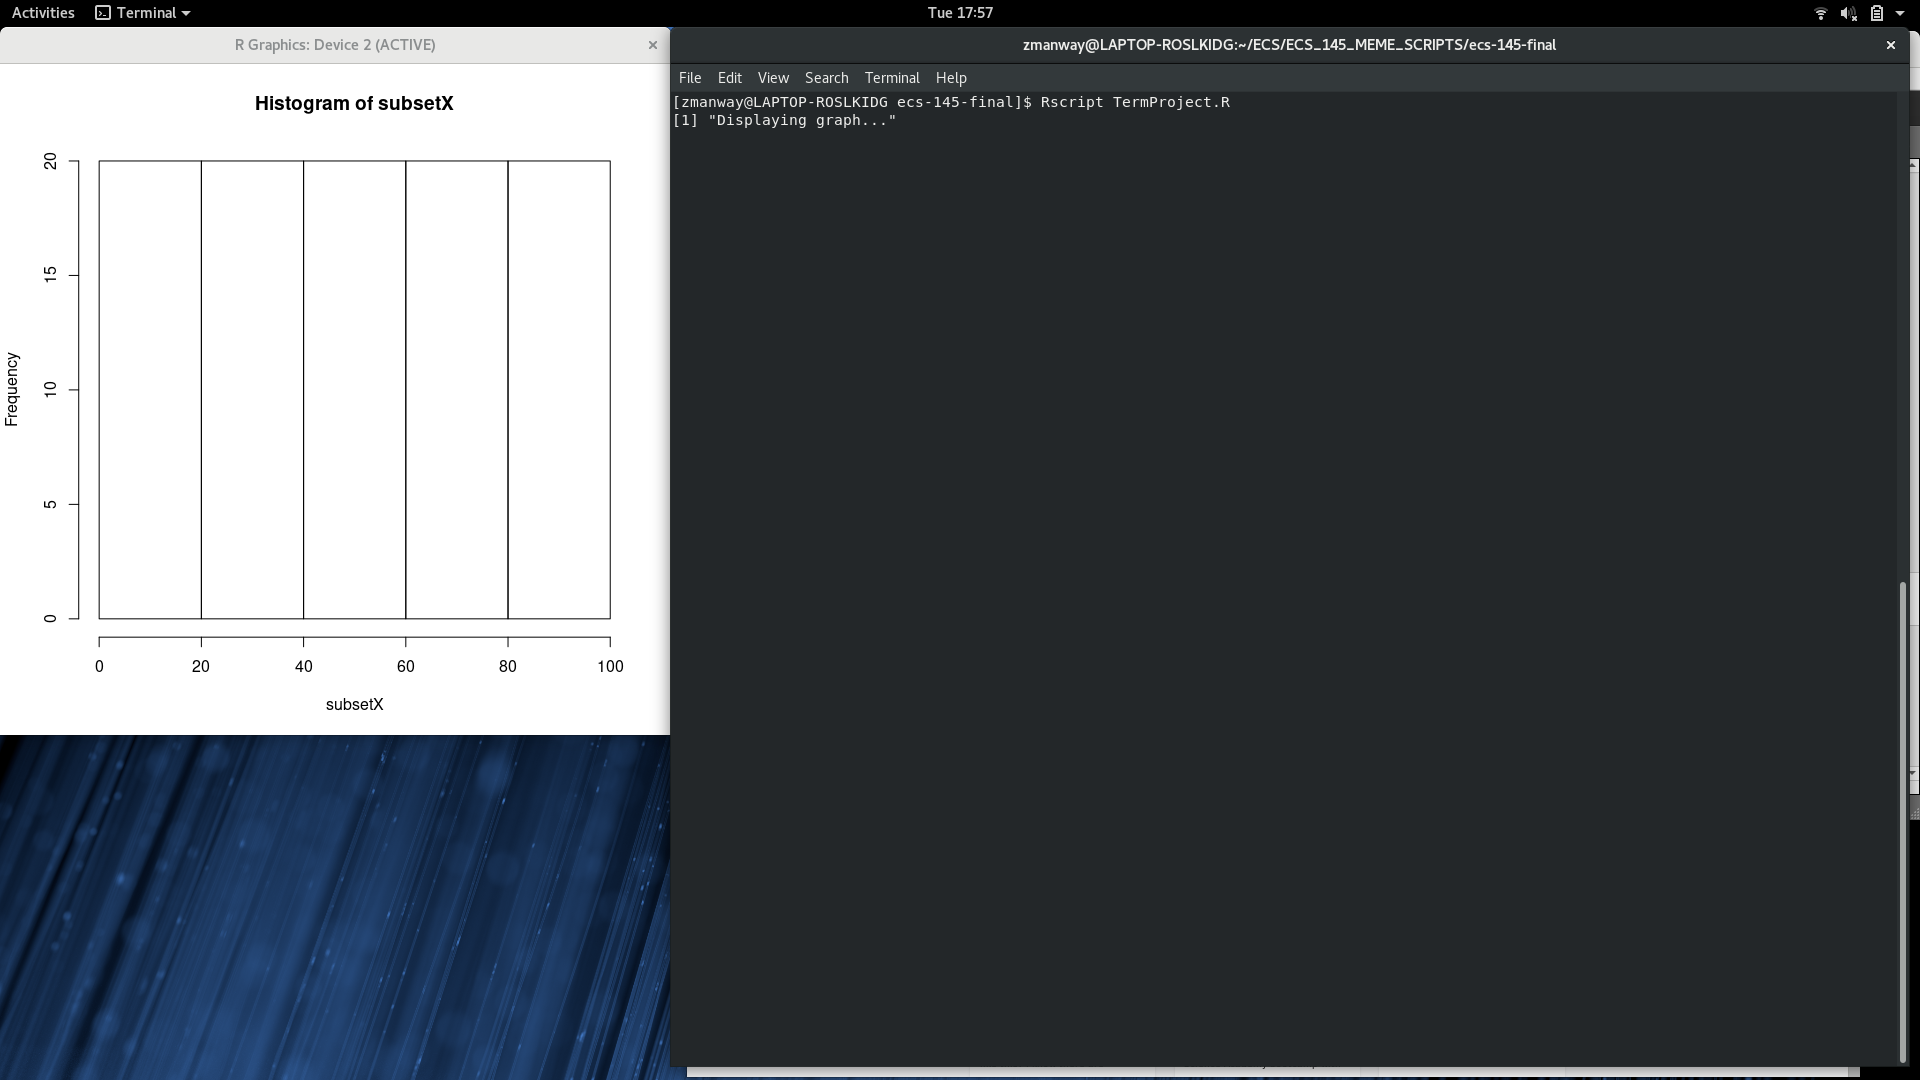
\includegraphics[width=\textwidth]{1.png}
\centering
\end{figure}

After pressing enter, we receive a prompt, giving us some options. Let's increase the number of buckets to 10. This will give us a graph, showing the previous graph with 5 buckets laid on top of it (note that if twoAtATime were false, the new graph would simply be displayed without the old one displayed with it).

\begin{figure}[H]
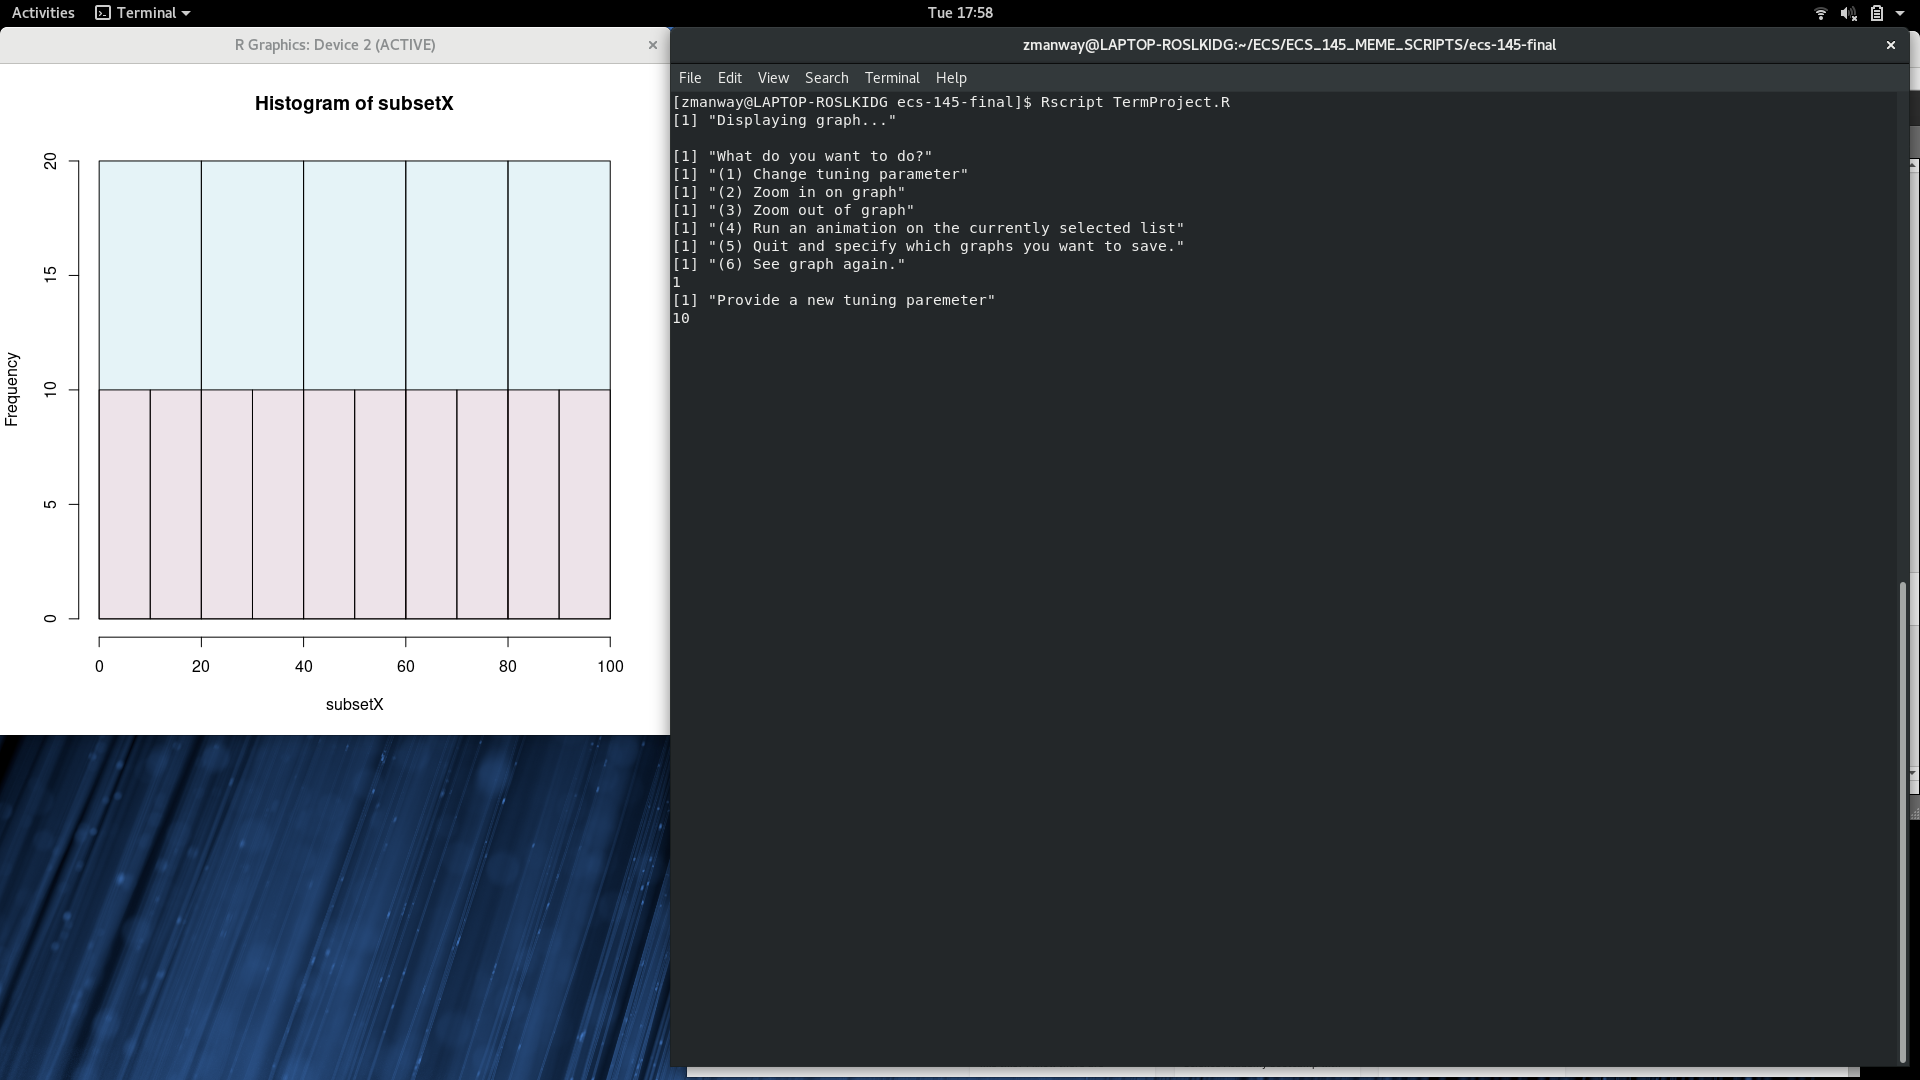
\includegraphics[width=\textwidth]{2.png}
\centering
\end{figure}


Upon pressing enter, we see the updated graph. We press enter again to get our prompt.

\begin{figure}[H]
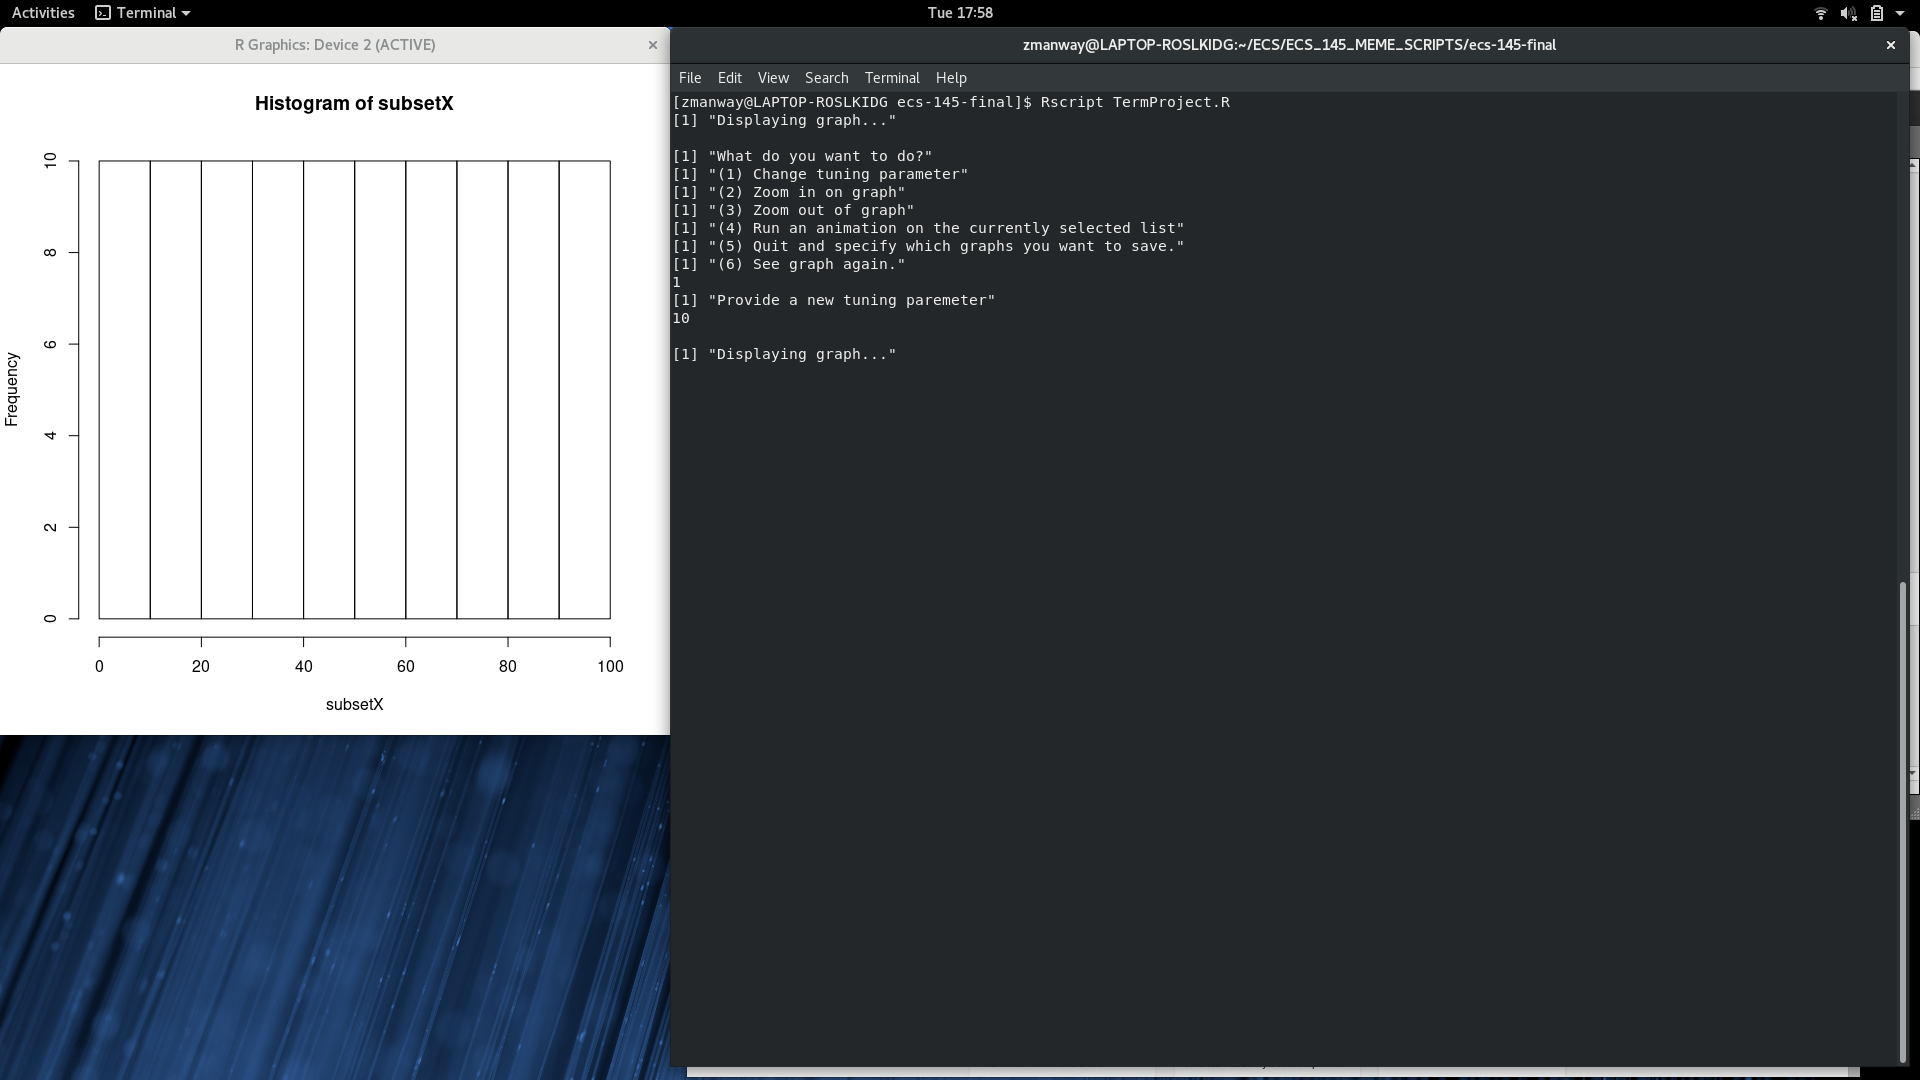
\includegraphics[width=\textwidth]{3.png}
\centering
\end{figure}

Now let's try to zooming in between data points at indices 25 and 75. This will give us a new graph.

\begin{figure}[H]
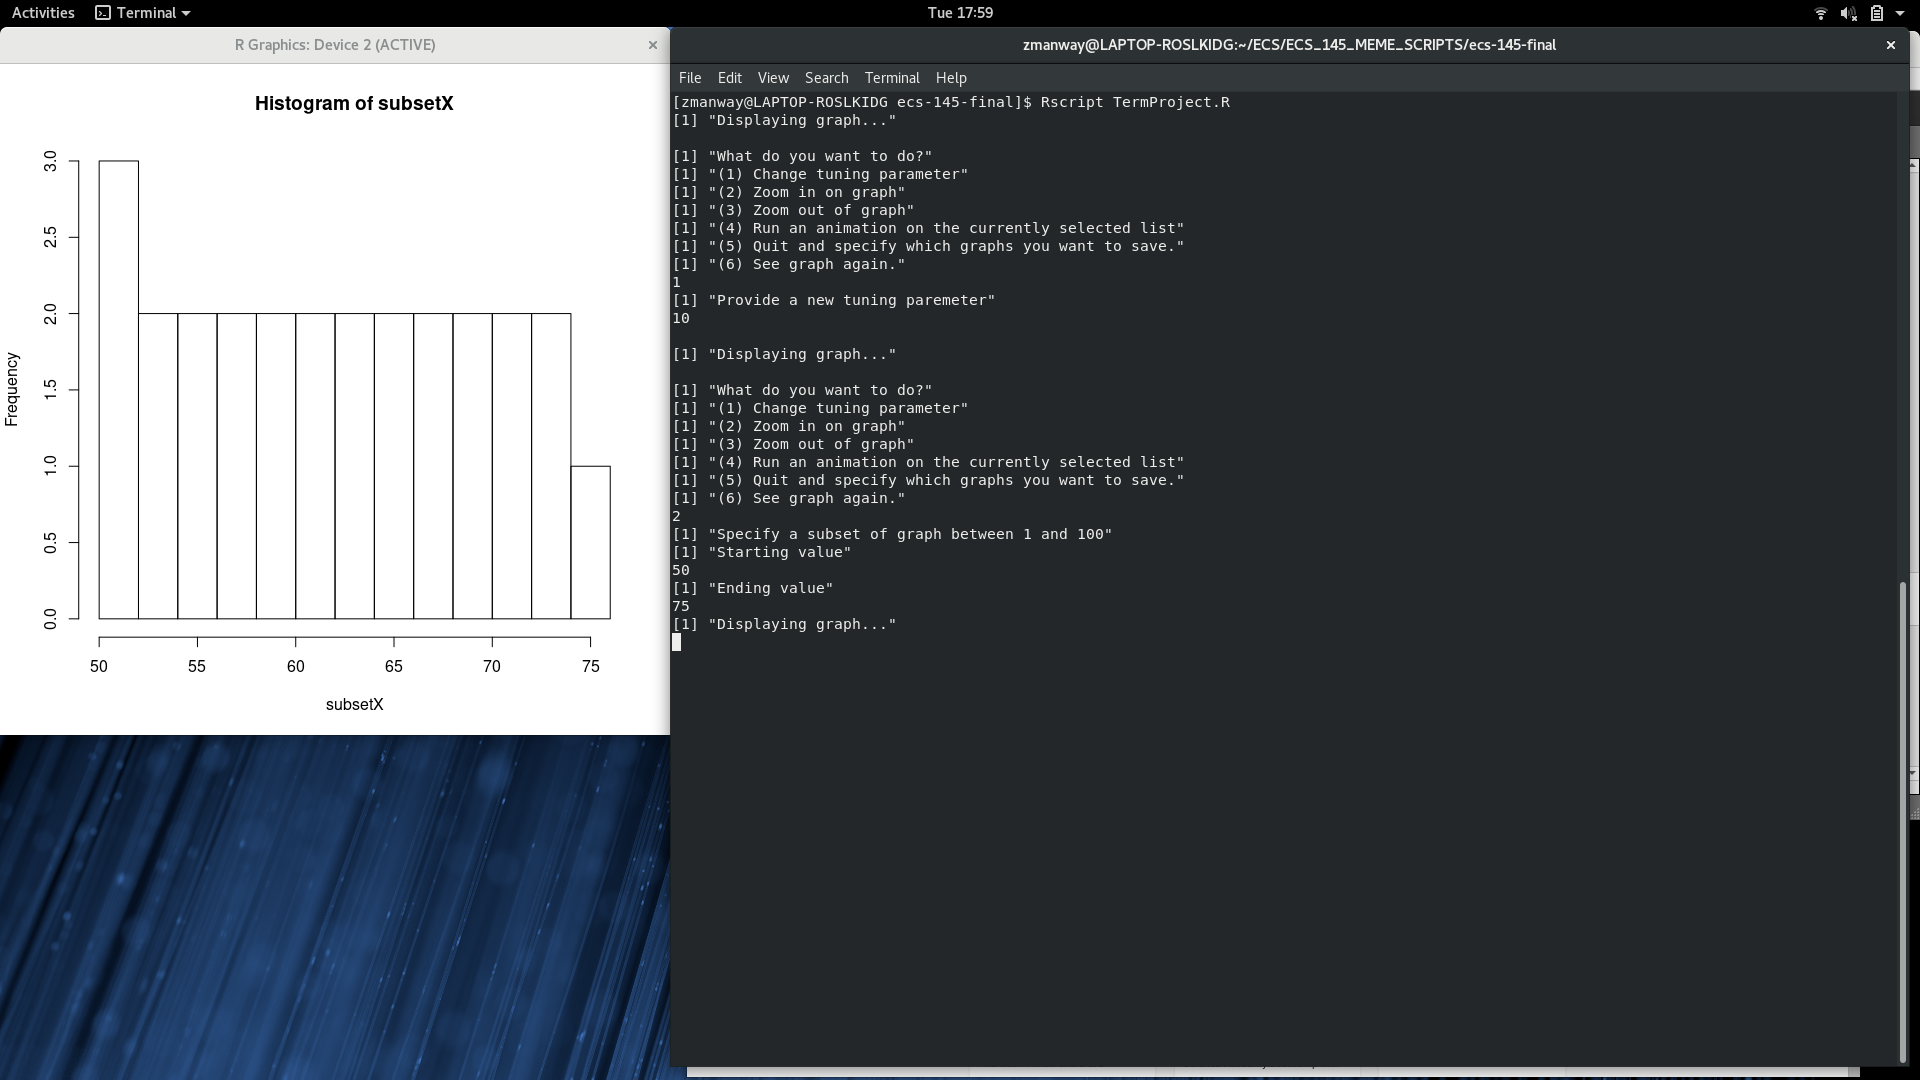
\includegraphics[width=\textwidth]{4.png}
\centering
\end{figure}

Press enter to get the prompt back. Now we can select option 3 to zoom out. We'll zoom out to the original selection of data. This can be done by selecting the 'y' option when prompted.

\begin{figure}[H]
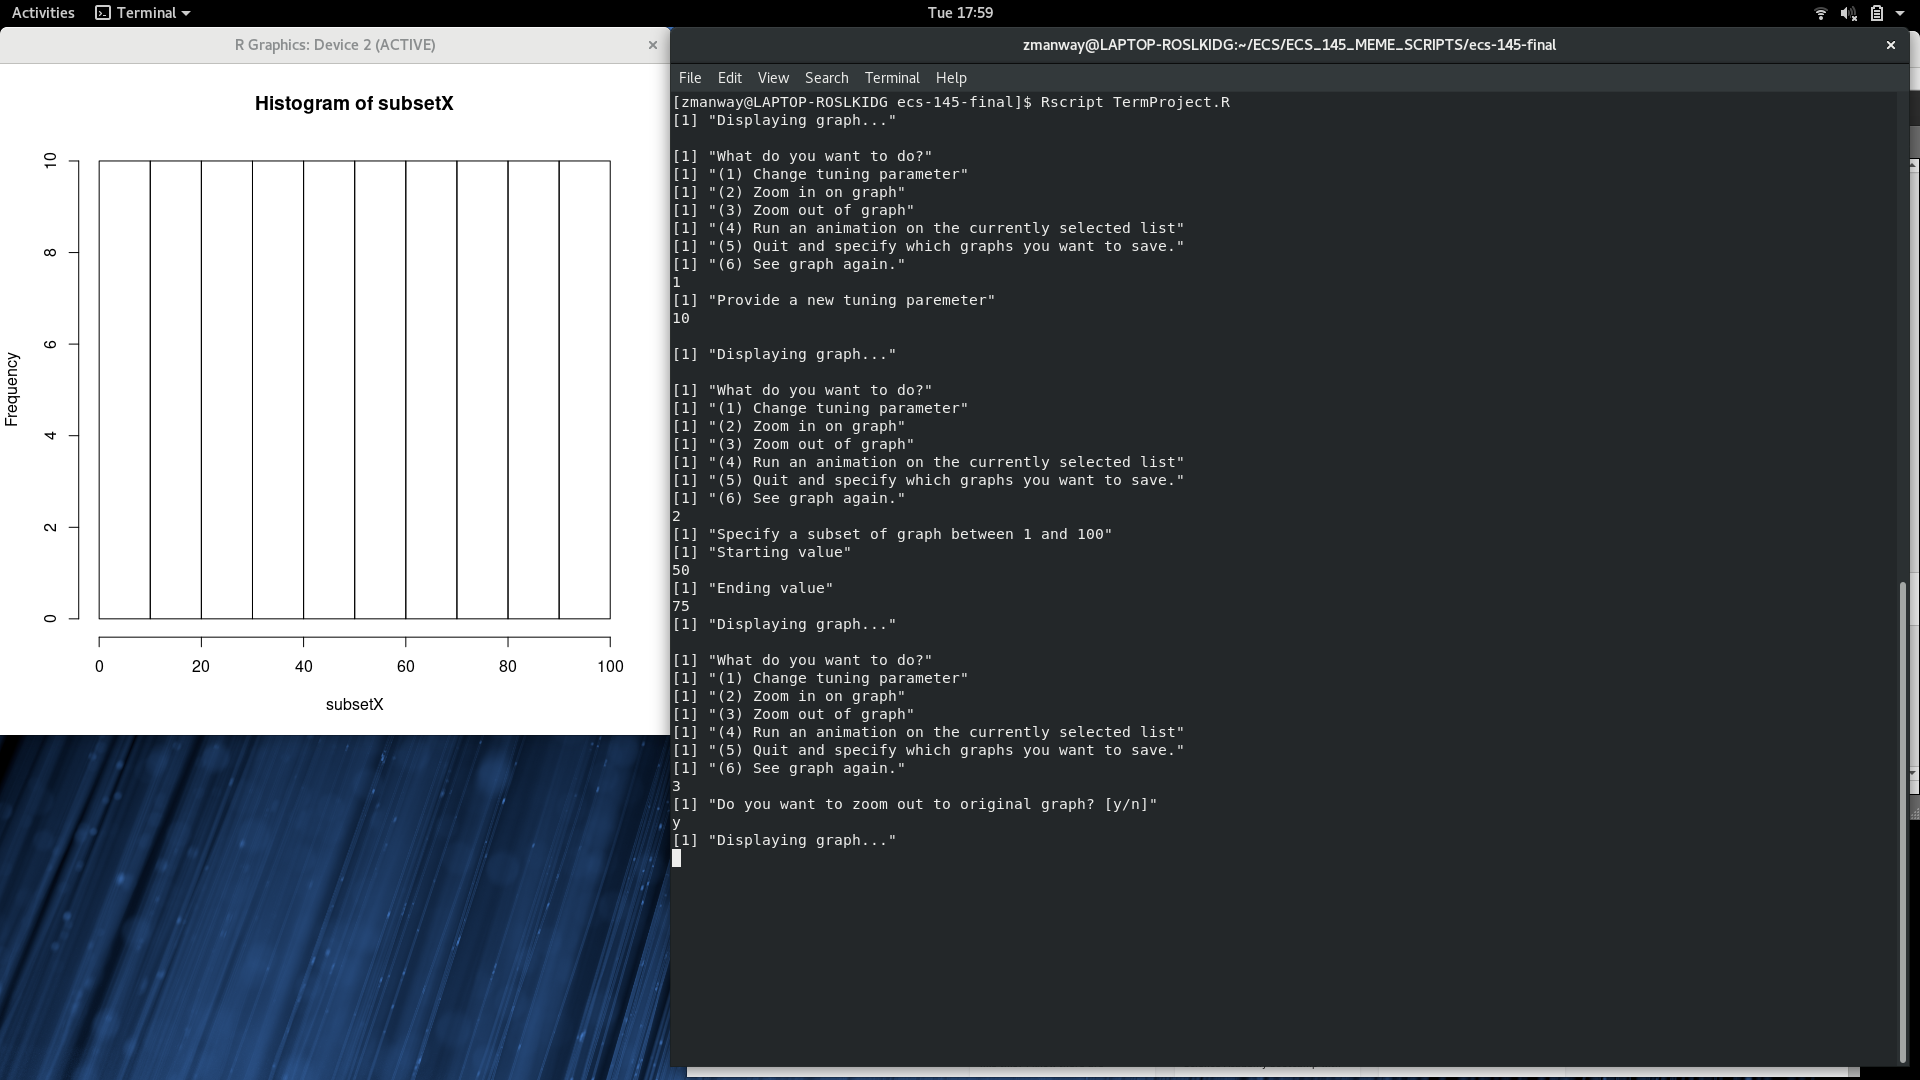
\includegraphics[width=\textwidth]{5.png}
\centering
\end{figure}

Finally, let's exit. We'll enter tunings 5, 10, and 20. After pressing 'q' to quit, the function terminates and returns an S3 object that supports plot, summary, and print.

\begin{figure}[H]
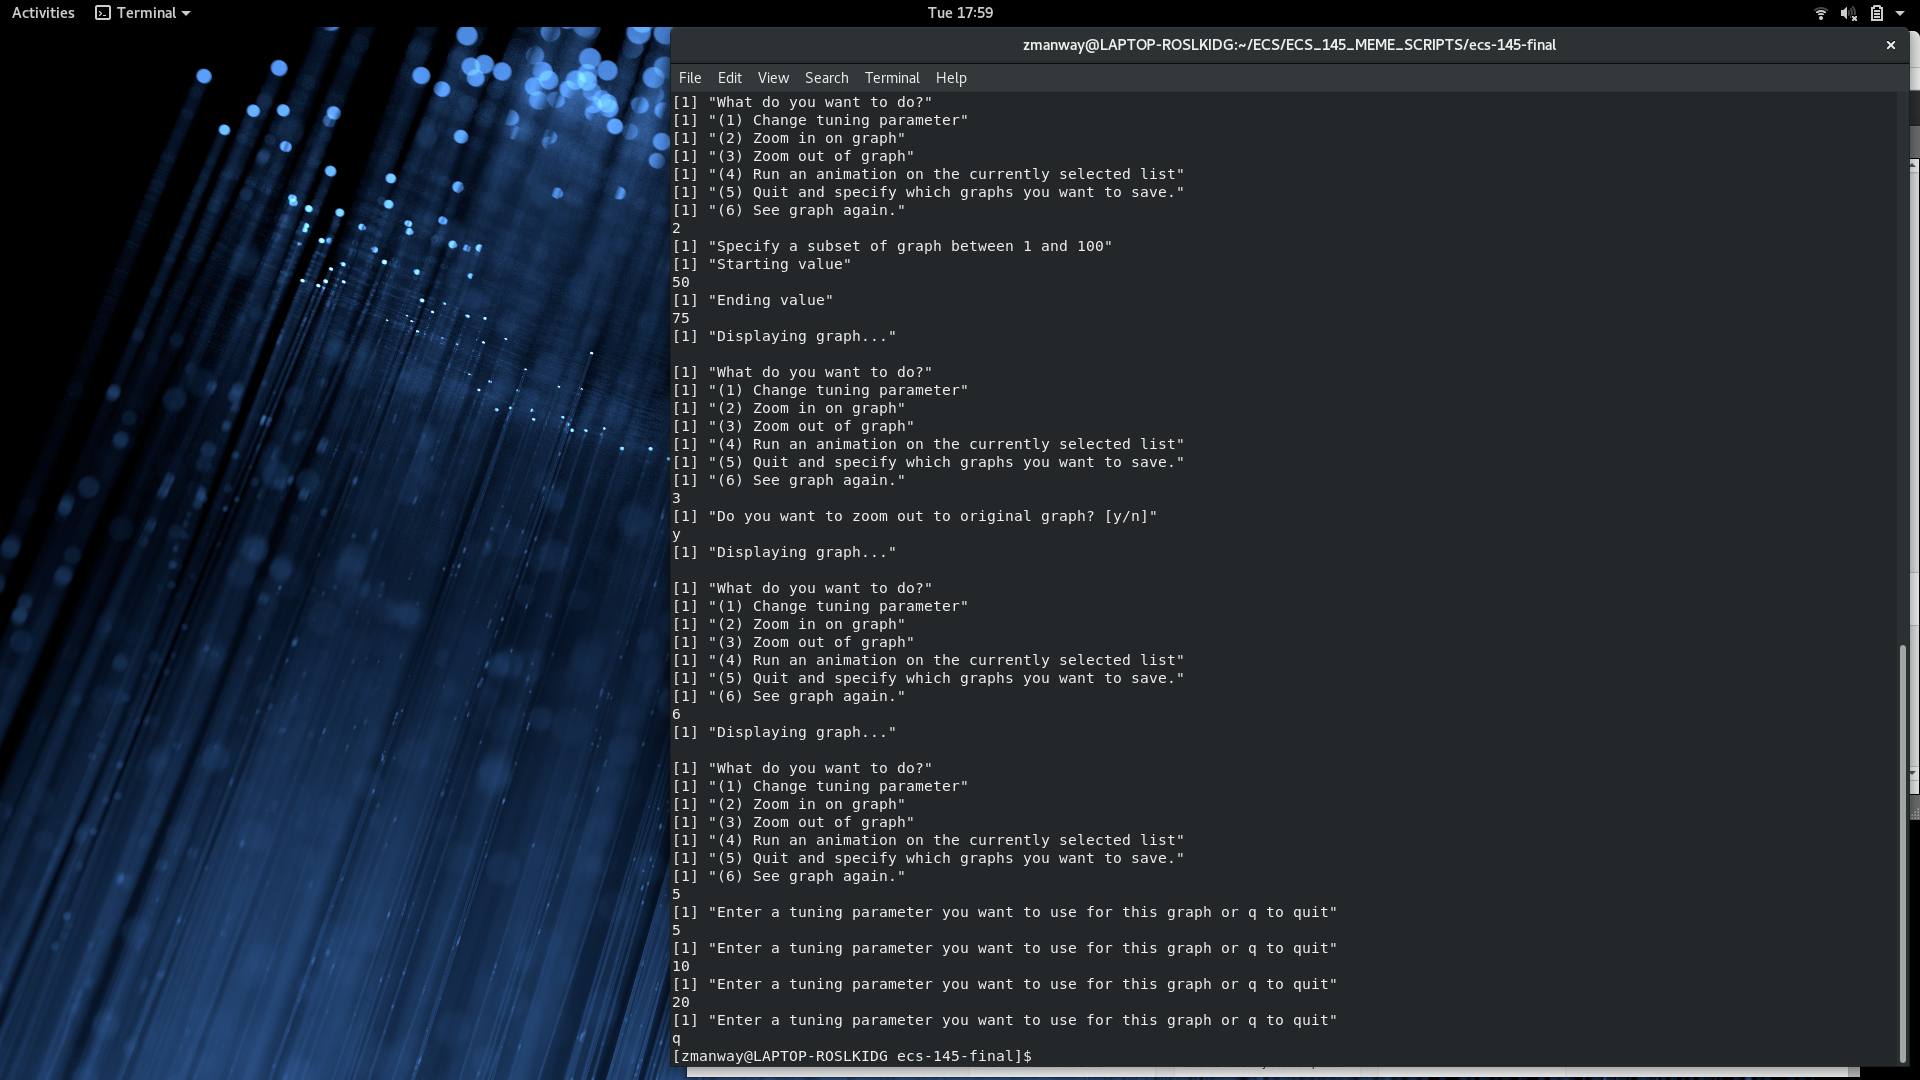
\includegraphics[width=\textwidth]{6.png}
\centering
\end{figure}

\section{Project Obstacles}
\subsection{Complications in gganimate}
We struggle collectively with getting gganimate to run. Zach ran into dependency issues when downloading on his computer (Fedora) based around non-existent C libraries. Atul struggled getting it to run on Windows. Jamie was eventually able to get it running on mac, and with some adjustments was able to get it to work on Windows and Linux as well.
\subsection{Refactoring}
After everyone finished their work, an aggressive refactor and merging period took place to combine everything. Everyone made some modification to the skeleton code to accommodate their work. This lead to some rather hairy merge conflicts. Zach was able to resolve them and everyone tested the final product repeatedly to make sure that all functionality was bug free.
\subsection{Graphics Drivers}
Another issues was figuring out how to configure graphics through Rscript. Eventually we figured out that X11 allowed for us to display graphs. Another issue we faced was that as soon as a graph opened, it would close instantly. We discovered that if the program waited for user input, the graph would stay open. This means that the driver will run until the enter key is pressed. Then graphics.off() can handle the window if it is still open.

\section{Group Contributions}
Everyone in this group made an honest and consistent effort to contribute. Below are everyone's contributions.\\
\subsection{Atul (The Idea/Solution Person)}
Atul consistently provided ideas on ways to improve the project as well as a means of implementing them. He facilitated a lot of discussion on Slack and was quick to find solutions to errors that were occurring. His key code contribution was his zooming implementation.
\subsection{Han (The Researcher)}
Han shined the most when we were doing our first coding session as a group. The rest of us would be scratching our heads trying to figure out how to do something and she would consistently be able to dig into the documentation and figure out how to do what we were trying to figure out. Her main code contribution was the overlaying of two graphs simultaneously.
\subsection{Jamie (The Implementer)}
Jamie was the only person who was able to figure out gganimate's documentation. In group settings, she was able to suggest potential fixes to issues, many of which were exactly what we needed. She was also helpful in catching errors and reading through the documentation during our second group meeting. Her main code contribution was the implementation of animations.
\subsection{Zach (The Outliner)}
Zach's main focus was setting up the project template, so that we could all convene and fill in all the pieces. He provided the skeleton for the project so that we just had to add the features in. He did the same thing for the report, so that everyone just had to fill in sections that applied to what they accomplished. His main code contribution was the implementation of the S3 object and its functions.\\\\
Everyone spent a similar amount of hours on the project and helped to fill out the report.

\section{Appendix}
\subsection*{TermProject.R}
\begin{lstlisting}[frame=single,language=R,showstringspaces=false]
## Package used to generate methods for displaying graphs
#install.packages("gganimate",dependencies=TRUE,
 repo="http://cran.rstudio.com/")
#install.packages("transformr", dependecies=TRUE, 
repo="http://cran.rstudio.com/")
library(ggplot2)
library(gganimate)
#library(transformr)


## GENERIC FUNCTIONS

## prints data of S3 object. Print of data vector is optional.
print.densEst <- function(obj, printVector = FALSE) {
   cat("Graph type is:",obj$estMethod,"\n")
   cat("Set of tunings are: ")
   print(obj$tunings)
   if (printVector) {
      cat("Data vector:\n")
      print(obj$dataVector)
   }
}

## plots function. Upon key press will close current graph and open next one
## until all are plotted.
plot.densEst <- function(obj) {
   if (length(obj$tunings) > 0) {
      for (i in 1:length(obj$tunings)) {
         X11()
         if (obj$estMethod == "hist") {
            hist(obj$dataVector, breaks = obj$tunings[i])
         }
         else {
            plot(density(obj$dataVector, bw = obj$tunings[i]))
         }
         readLines(file("stdin"), 1)
         graphics.off()
      }
   }
}

## prints some basic statistical data about the data set, its est method
## and some stats about the density
summary.densEst <- function(obj) {
   cat("Estimation method: ")
   print(obj$estMethod)
   if (length(obj$dataVector) > 0) {
      print(paste("Mean of dataset:",mean(obj$dataVector)))
      print(paste("Standard deviation of dataset:",sd(obj$dataVector)))
   }
   if (length(obj$tunings)) {
      print(paste("Mean of bins:",mean(obj$tunings)))
      print(paste("Standard deviation of bins",sd(obj$tunings)))
   }
}


## HELPERS

## when two at a time, allows for displaying graphs two at a time
overlayGraphs <- function(subsetX, estMethod, graph, tuning) {
   X11()
   # DENSITY OVERLAY
   if (estMethod == "density") {
      newGraph <- density(subsetX, bw=tuning)
      currentGraph <- graph
      xlim <- c(-2000,2000)
      ylim <- range(currentGraph$y, newGraph$y)
      plot(currentGraph$x, currentGraph$y, col = 1, lwd = 2,
           type = "l", xlim = xlim, ylim = ylim,
 main="Superimposed Density Plot",xlab="x-axis",ylab="y-axis")
      lines(newGraph$x, newGraph$y, col = 2, lwd = 2)
   }
     
   # HISTOGRAM OVERLAY
   else if (estMethod == "hist") {
      newGraph <- hist(subsetX, breaks=tuning)
      currentGraph <- graph
      xlim <- range(currentGraph$breaks, newGraph$breaks)
      ylim <- c(0,max(c(currentGraph$count, newGraph$count)))
      plot(currentGraph, col = rgb(173,216,230,max = 255, alpha = 80,
           names = "lt.blue"), xlim = xlim, ylim = ylim, 
main="Superimposed Histogram",xlab="x-axis",ylab="y-axis")
      plot(newGraph, add=TRUE,
           col = rgb(255,192,203, max = 255, alpha = 80,
                     names = "lt.pink"))
   }
   ## wait for keystroke before closing
   buffer <- readLines(file("stdin"), 1)
   graphics.off()
}

## returns S3 object that represents list of data with defined estMethod that
## can be displayed with a variety of tunings
getFinalGraphs <- function(x, estMethod) {
   ## S3 object requires 3 components:
   ## 1) The dataset x
   ## 2) The estimation method
   ## 3) The set of tunings
   
   thisEnv <- environment()
   
   ## get tuning list
   tunings <- c()
   while (TRUE) {
      print("Enter a tuning parameter you want
 to use for this graph or q to quit")
      tuning <- readLines(file("stdin"), 1)
      if (tuning == "q") {
         break
      }
      else if (is.na(as.integer(tuning))) {
         print("Tuning must be a non-negative integer")
      }
      else {
         tunings <- c(tunings, as.integer(tuning))
      }
   }

   ## create S3 obj
   obj <- list (
      dataVector = x,
      tunings = tunings,
      estMethod= estMethod
   )

   assign('this',obj,envir=thisEnv)
   class(obj) <- "densEst"
   return(obj)
}

## grabs values and runs animations based on supplied
runAnimation <- function(x, estMethod) {
   print("Specify a starting tuning value ")
   start_tuning <- as.integer(readLines(file("stdin"), 1))
   print("Specify a ending tuning value")
   end_tuning <- as.integer(readLines(file("stdin"), 1))

   X11()
   if (estMethod == 'hist') {
      h <- hist(x, breaks = start_tuning, plot = FALSE)
      df <- as.data.frame(cbind(ds = start_tuning, 
xs = h$mids, ys = h$counts))

      for (i in start_tuning+1:end_tuning) {
        h2 <- hist(x, breaks = i, plot = FALSE)
        df2 <- as.data.frame(cbind(ds = i, 
xs = h2$mids, ys = h2$counts))
        df <- rbind(df, df2)
        df <- as.data.frame(df)
      }
      plt <- ggplot(data=df, aes(x=xs, y=ys)) +
 geom_bar(stat="identity") + transition_states(ds, transition_length = 1, 
state_length = 1, wrap = FALSE) + labs(title =
 'Bins: {closest_state}') + xlab("X Values") + ylab("Y Values")
      print(plt)
   }
   else {
      d1 <- density(x, bw =  start_tuning)
      d2 <- density(x, bw = end_tuning)
      df1 <- as.data.frame(cbind(ds = 1, xs = d1$x, ys = d1$y * d1$n))
      df2 <- as.data.frame(cbind(ds = 2, xs = d2$x, ys = d2$y * d2$n))
      m <- merge(x = df1, y = df2, all = TRUE)
      plt <- ggplot(m, aes(x = xs, y = ys)) + geom_line() +
 transition_states(ds, transition_length = 1, 
state_length = 1, wrap = FALSE) + 
labs(title = 'Changing Bandwidth') + xlab("X Values") + ylab("Y Values")
      print(plt)
   }
}

## returns boolean based on if vec args is greater than start, less than end
subset <- function(vec,start,end)
{
   if (vec >= start & vec <= end) return(TRUE) else return(FALSE)
}

getSubset <- Vectorize(subset)

## grabs subset of graph and returns it
zoomIn <- function(x, subsetX) {
   valid_index <- 0
   while(valid_index == 0)
   {
      print(paste("Specify a subset of graph between",range(subsetX)[1],
      "and",range(subsetX)[2]))
      print("Starting value")
      start_index <- as.integer(readLines(file("stdin"), 1))
      if (start_index < range(subsetX)[1])
      {
         print("Invalid. Starting value should be larger.")
         next
      }
      print("Ending value")
      end_index <- as.integer(readLines(file("stdin"), 1))
      if(end_index > range(subsetX)[2])
      {
         print("Invalid. Ending value should be smaller.")
         next
      }
      if(end_index == start_index)
      {
         cat("Invalid range. Max value cannot be the 
same as min value. Please reenter indices.\n")
         next
      }
      else if (end_index < start_index)
      {
         cat("Invalid range. Max value cannot be 
smaller than min value. Please reenter indices.\n")
         next
      }
      valid_index <- 1
   }
   ## display graph of subset
   return(x[getSubset(x,start_index,end_index)])
}

## handles zooming out graph
zoomOut <- function(x, subsetX)
{
   if(range(x)[1] == range(subsetX[1]) && range(x)[2] == range(subsetX)[2])
   {
      print("Cannot zoom out. Graph is in original state.")
      return(x)
   }
   else
   {
      print("Do you want to zoom out to original graph? [y/n]")
      response <- readLines(file("stdin"),1)
      if (response == "y" || response == "Y")
      {
         return(x)
      }
      else if (response == "n" || response == "N")
      {
         valid_index <- 0
         while (valid_index == 0)
         {
            print(paste("Specify a subset of graph between",range(x)[1],
            "and",range(x)[2]))
            print("Start index")
            start_index <- as.integer(readLines(file("stdin"), 1))
            if (start_index > range(subsetX)[1])
            {
               print("Invalid. Starting index should be smaller.")
               next
            }
            print("End index")
            end_index <- as.integer(readLines(file("stdin"), 1))
            if (end_index < range(subsetX)[2])
            {
               print("Invalid. Ending index should be larger.")
               next
            }
            if(end_index == start_index)
            {
               cat("Invalid range. Max value cannot
 be the same as min value. Please reenter indices.\n")
               next
            }
            else if (end_index < start_index)
            {
               cat("Invalid range. Max value cannot 
be smaller than min value. Please reenter indices.\n")
               next
            }
         valid_index <- 1
         }
         ## display graph of subset
         return(x[getSubset(x,start_index,end_index)])
      }
   }
}

## grabs and returns new tuning paremeter from user. Validates input before
## returning.
getNewTuningParameter <- function() {
   while(TRUE) {
      print("Provide a new tuning paremeter")
      tuning <- as.integer(readLines(file("stdin"), 1))
      if (is.na(tuning) || tuning < 1) {
         print("Tuning must be a non-negative integer")
      }
      else {
         return(tuning)
      }
   }
}

## Grab user input to see what action they want to do. Returns integer that
## corresponds with requested action. Input guaranteed to be valid,
## as function will validate input and ask user until valid input provided.
grabUserRequest <- function() {
   while(TRUE) {
      print("What do you want to do?")
      print("(1) Change tuning parameter")
      print("(2) Zoom in on graph")
      print("(3) Zoom out of graph")
      print("(4) Run an animation on the currently selected list")
      print("(5) Quit and specify which graphs you want to save.")
      print("(6) See graph again.")
      input <- readLines(file("stdin"), 1)

      if (is.na(as.integer(input)) || as.integer(input) < 1 ||
          as.integer(input) > 6) {
         print("Invalid choice...")
      }
      else {
         return(as.integer(input))
      }
   }
}

## Used to explore potential curves of a dataset
## , allowing for iterative testing by the user. 
## Will save graphs that user wants.
## Args:
## x (Vector): numeric vector to be graphed
## estMethod (string): Type of method. Should be 'hist' or 'density'
## tuning: breaks or bw, based on estMethod
exploreShape <- function(x,estMethod,tuning,twoAtATime) {
   ## subset of graph we are graphing. Be default is the entire graph
   subsetX <- x

   while (TRUE) {
      ## Allow user to view plot until they close the window
      X11()
      print("Displaying graph...")
      if (estMethod == 'hist') {
	  # global instance allows overlays
         graph <<- hist(subsetX, breaks = tuning) 
         plot(graph, main="Histogram of Current Numeric Vector", 
xlab="x-axis",ylab="y-axis")
      }
      else {
         graph <<- density(subsetX, bw = tuning)
         plot(graph, main="Density Plot of Current Numeric Vector",
xlab="x-axis",ylab="y-axis")
      }
      
      buffer <- readLines(file("stdin"), 1)
      graphics.off()
      ## once closed, see what the user want to do
      input <- grabUserRequest()
      if (input == 1) {
         tuning <- getNewTuningParameter()

         ## handle plotting overlays
         if (twoAtATime) {
            overlayGraphs(subsetX, estMethod, graph, tuning)
         }
      }
      else if (input == 2) {
         subsetX <- zoomIn(x, subsetX)
      }
      else if (input == 3) {
         subsetX <- zoomOut(x, subsetX)
      }
      else if (input == 4) {
         runAnimation(x, estMethod)
         while (!is.null(dev.list())) Sys.sleep(1)
      }
      else if (input == "5") {
         return(getFinalGraphs(x, estMethod));
      }
      else if (input == 6) {
         next
      }
   }
}

\end{lstlisting}

\end{document}
